\chapter{Regul�re Grammatik}

\section{Definition}

\subsection{Definition einer Grammatik}

Eine Grammatik G =(T,N,P,S) besteht aus:

\begin{tabular*}{1.0\textwidth}{l @{\extracolsep{\fill}} l}

T & einer Menge von Terminalsymbolen (kurz Terminalen)\\
N & einer Menge von Nichtterminalsymbolen (kurz Nichtterminale)\\
 & T und N sind disjunkte Mengen\\
 S $\in$ N & einem Startsymbol aus der Menge der Nichtterminale\\
 P $\subseteq$ N $\times$ V* & Menge der Produktionen; (A,x) $\in$ P, A $\in$ N
 und x $\in$ V*; \\
  & statt (A,x) schreibt man A $\rightarrow$ x\\
 V=T $\cup$ N & hei�t Vokabular, seine Elemente hei�en Symbole\\
 
\end{tabular*}

\subsection{Definition einer rechtslinearen Grammatik}

Eine rechtslineare Grammatik G=G(T,N,P,S) ist einer rechtslineare Grammatik,
wenn sie folgenden Anforderungen gen�gt:

X $\rightarrow$ aY \\
X $\rightarrow$ a \\
X $\rightarrow$ $\varepsilon$ \\
mit X,Y $\in$ N und a $\in$ T \\

\section{Datenstruktur}

\subsection{Implementation}

\begin{figure}[h]
  \begin{center}
  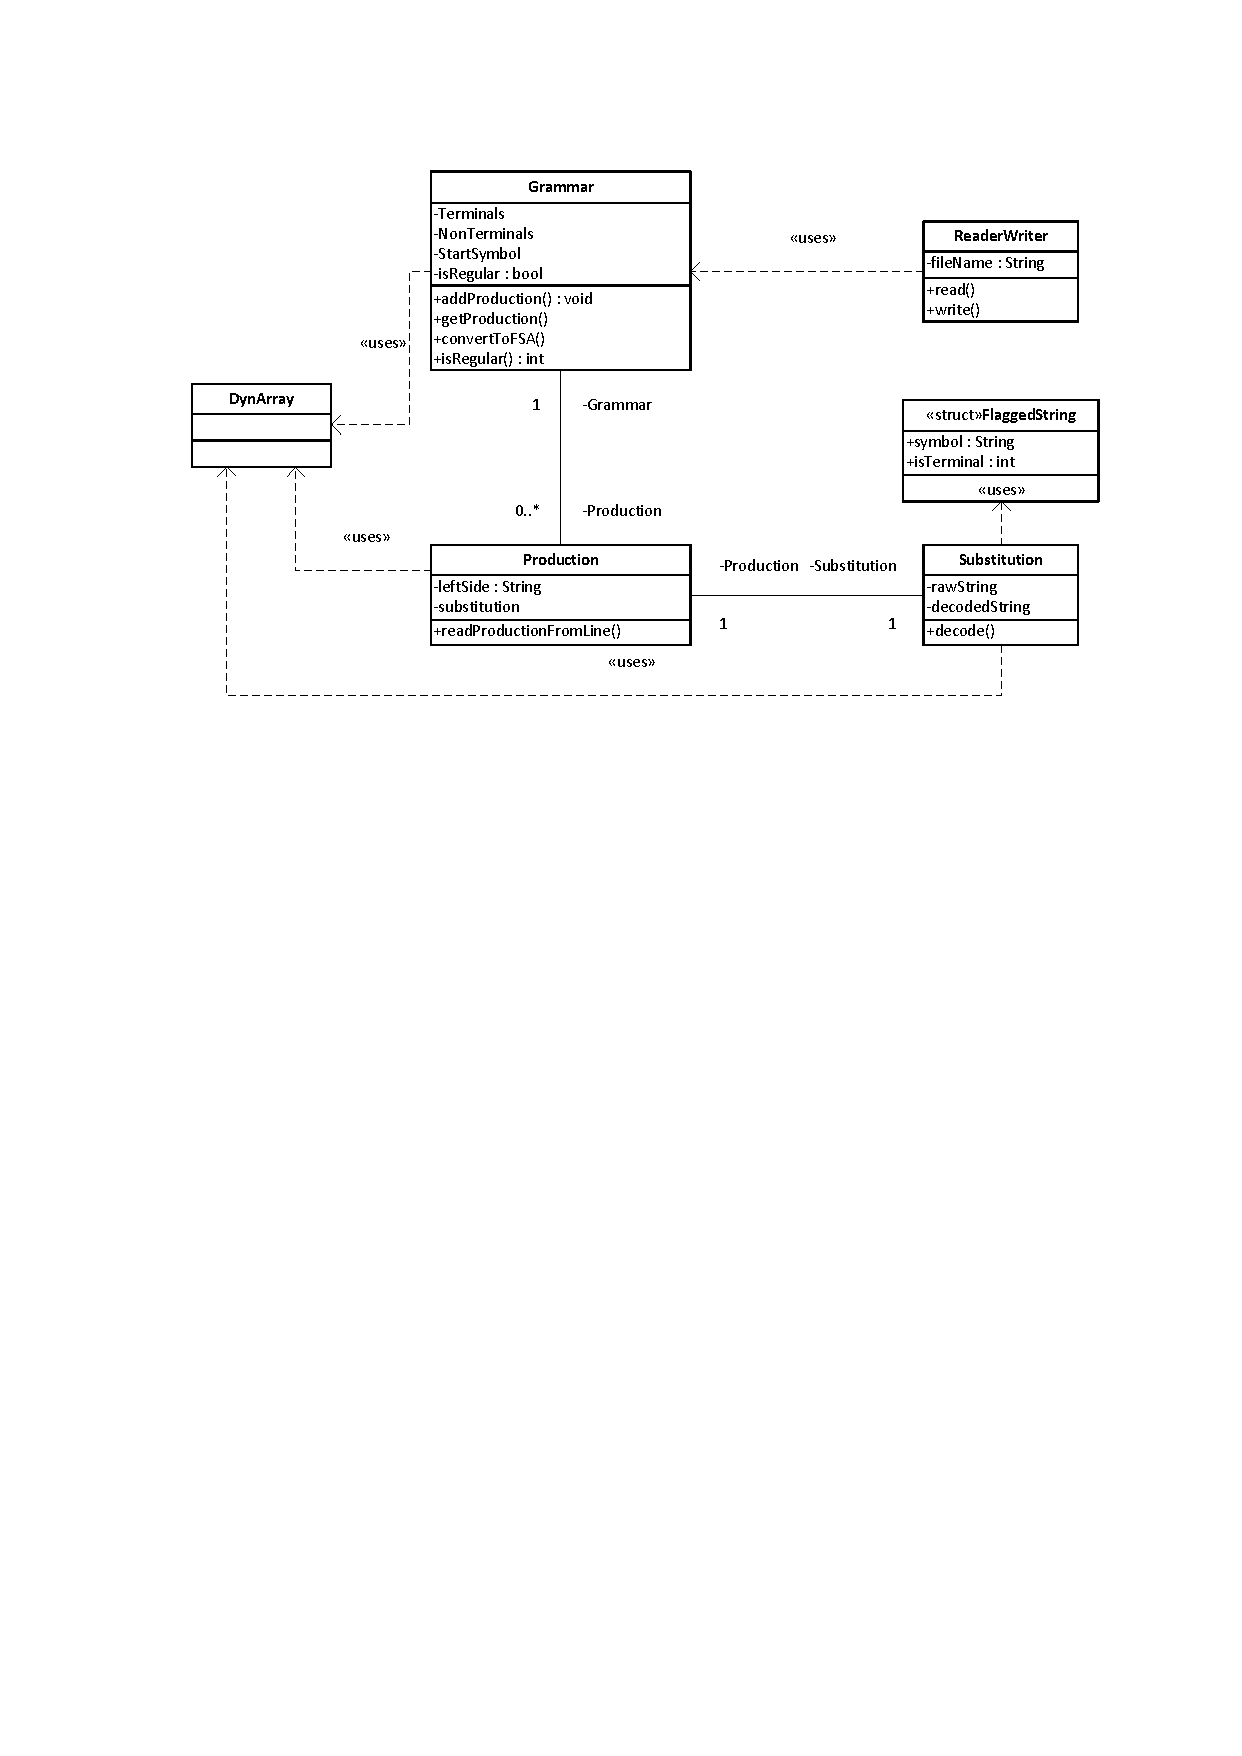
\includegraphics[scale=0.95]{objectsToInclude/UMLGrammar.pdf}
  \caption{Regul�re Grammatik UML Diagramm}
  \label{fig:UMLRegGrammar}
  \end{center}
\end{figure}

Die Klasse \textit{Grammar} besteht aus zwei \textit{dynArrays}
\textit{Terminals} und \textit{NonTerminals}, in diesen werden alle Terminal- und Nichtterminalsymbole
als String gespeichert, einem String \textit{Startsymbol} f�r das Startsymbol
der Grammatik, einer Integer Variablen isRegular, die angibt ob die Grammatik
regul�r ist und einem weitern \textit{dynArray} \textit{Productions} f�r die
Produktionen. Die Template-Klasse \textit{dynArray} erm�glicht eine unbekannte
Anzahl von Variablen in einem Feld zu speichern, auf die Inhalte des Feldes
wird mit dem [ ]-Operator zugegriffen.

Produktionen bestehen aus einem Nichtterminal auf der linken Seite und eine
Substitution auf der rechten Seite des Pfeils. Die Klasse \textit{Production}
setzt sich aus einer Stringvariablen f�r die linke Seite und einer Klasse
Substitution f�r die rechte Seite zusammen.

Die Klasse \textit{Substitution} enth�lt eine Zeichenkette \textit{rawString}.
In dieser wird eine unbearbeitet Substitution abgespeichert, also zum Beispiel
direkt nach dem Einlesen, bevor diese dann weiter verarbeitet wird. In einem
\textit{dynArray} vom Typ \textit{flaggedString} wird dann die vollst�ndig
verarbeitete Substitution ,unter dem Namen \textit{decodedSubstitution},
gespeichert. Der Struct \textit{flaggedString} setzt sich aus einem Integer,
der angibt ob das Symbol ein Terminal ist oder nicht und einem String, der das
Symbol speichert, zusammen. Die Funktion \textit{decode} wandelt nun den
\textit{rawString}, eine Folge von Terminalen und Nichtterminalen, in ein
flaggedString Array um, zur Weiterverarbeitung.

\section{Einlesen von regul�ren Grammatiken}

\section{Konvertierungen}

\subsection{Konvertierung zu einem endlichen Zustandsautomaten}

\section{Minimierung eines endlichen Zustandsautomaten}